\chapter{Introduction}
\label{chap_intro}

Mobile cellular networks beyond fifth and sixth-generation wireless systems (5G and 6G) are set to provide connectivity not only to end-users with improved capabilities, but also to different types of devices such as buildings, vehicles, and appliances.
Although the focus of 5G is on connecting devices from the Internet of Things (IoT) and helping to automate industrial systems, 6G aims to unify the human experience across the physical, digital, and human world \cite{6G-explained-NOKIA}.

% TODO: search image from Thorsten's article

\begin{figure}[H]
    \centering
    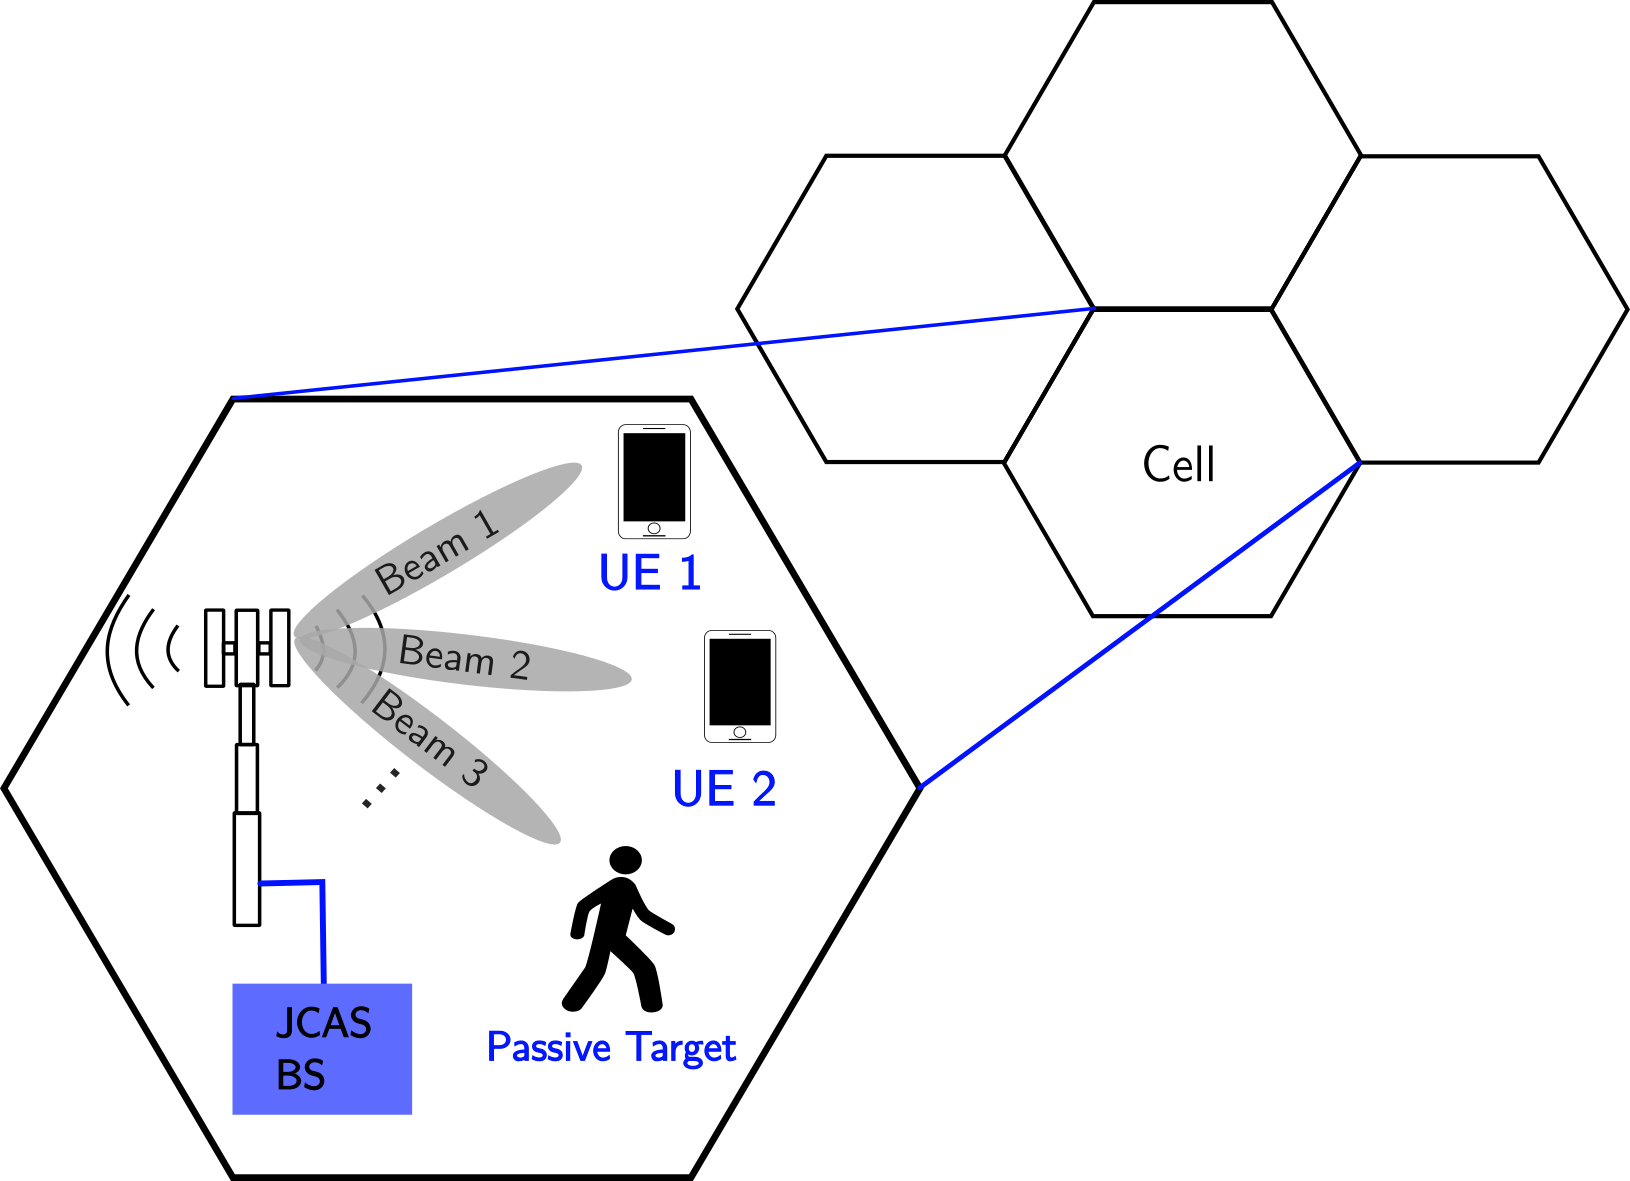
\includegraphics[width=0.7\textwidth]{Images/introduction/isac-scheme-1.png}
    \caption{Illustration of an ISAC scenario.}
    \label{fig:isac-scheme-1}
\end{figure}

6G will build on top of 5G and 5G-Advanced systems and use cases, driving their adoption through optimization and cost reduction. Nonetheless, new use-cases will be defined and enabled by the network's new abilities.

Thanks to the massive deployment of connected sensors and artificial intelligence (AI/ML) it will be possible to generate digital twins capable of real-time updates and prediction.  Digital twin models are essential for understanding what is occurring in the real world, predicting potential results, forecasting needs, and taking effective measures.

One of the most notable advancements in 6G technology will be the ability to perceive the surrounding environment, including people and objects, called network sensing. This capability converts the network into a source of valuable situational data by capturing and interpreting signals reflected by various entities. Determining characteristics such as type, shape, relative position, speed, and even material properties, advanced sensing empowers the creation of true-to-model digital twins. Moreover, when this data is fused with information from other sensors, artificial intelligence and machine learning, it unlocks new insights from the physical world, enhancing the network's cognitive abilities.

\section{Thesis contribution}

\section{Thesis outline}
